% Dans l'introduction, on présente le problème étudié et les buts
% poursuivis. L'introduction permet de faire connaître le cadre de la
% recherche et d'en préciser le domaine d'application. Elle fournit
% les précisions nécessaires en ce qui concerne le contexte de
% réalisation de la recherche, l'approche envisagée, l'évolution de
% la réalisation. En fait, l'introduction présente au lecteur ce
% qu'il doit savoir pour comprendre la recherche et en connaître la
% portée.

\Chapter{INTRODUCTION}\label{sec:Introduction} 

The growing accessibility to robots has enabled the rise of a new field of robotic called swarm robotics. Such multi-robot systems are characterized by their ability to adapt to changing quantities of robots, the incompetence of the entities when considered individually and by the decentralized environment in which they evolve \cite{sahin2005swarm}. This new field of robotics has been widely inspired by insects, where impressive results are achieved by combining efforts through self organization in the pursuit of a common goal. Robot swarms are particularly appealing for exploration missions involving large and unknown environments where a team effort can yield better results.

Swarm systems should in theory be less prone to failures because of their inherent redundancy. However, it has been demonstrated that in practice, they do not benefit of this property and are, in some cases, even less reliable than traditional centralized robots systems in the presence of risk. It has been shown that individual failures often lead to the complete system failure, challenging the assumption that swarm systems are robust by nature \cite{bjerknes2013fault}. Designing specific tools for risk management in swarm systems is therefore of high importance \cite{prorok2021beyond}. The two algorithms DORA-Explorer and RASS that will be presented in the thesis are a step in this direction and aim at improving tolerance to risk in swarm exploration.

\section{Definitions and Basic Concepts}
The basic concepts upon which the two algorithms DORA-Explorer and RASS are built will be presented in the following section. 

\subsection{Swarm Intelligence}
Swarm intelligence is a discipline that focuses on the mechanisms leading to global order in systems composed of many individuals coordinating between each other through only local interactions. Swarm intelligence can be seen in both natural and artificial systems where the collective behaviors are obtained in a fully decentralized fashion. Many examples of such systems can be found in nature, for example colonies of ants, schools of fish, flocks of birds or herds of land animals \cite{Dorigo:2007}. Systems that fall into the discipline of swarm intelligence display the following characteristics: 

\begin{itemize}
    \item A swarm system comprises many individuals and should be able to adapt to varying quantities of individuals
    \item There is no central coordination, the behaviors of the agents emerge solely from local interactions
    \item The system is greater than the sum of its individuals. In other words, when taken individually, the agents are relatively incapable but collectively they achieve impressive results   
\end{itemize}

Such characteristics result in an adaptable system that should display better tolerance to faults. Indeed, the absence of central coordination not only eliminates a bottleneck that could limit scalability, it also removes a central point of failure that could compromise the entire system if taken down.

\subsection{Swarm Robotics}
\label{sec:designprinciples}
Swarm robotics falls into the artificial category of swarm intelligence and more specifically corresponds to the application of the discipline to the field of robotics. It is at the intersection of collective robotics and swarm intelligence as shown in figure \ref{venne}. 

\begin{figure}[h]
    \centering
    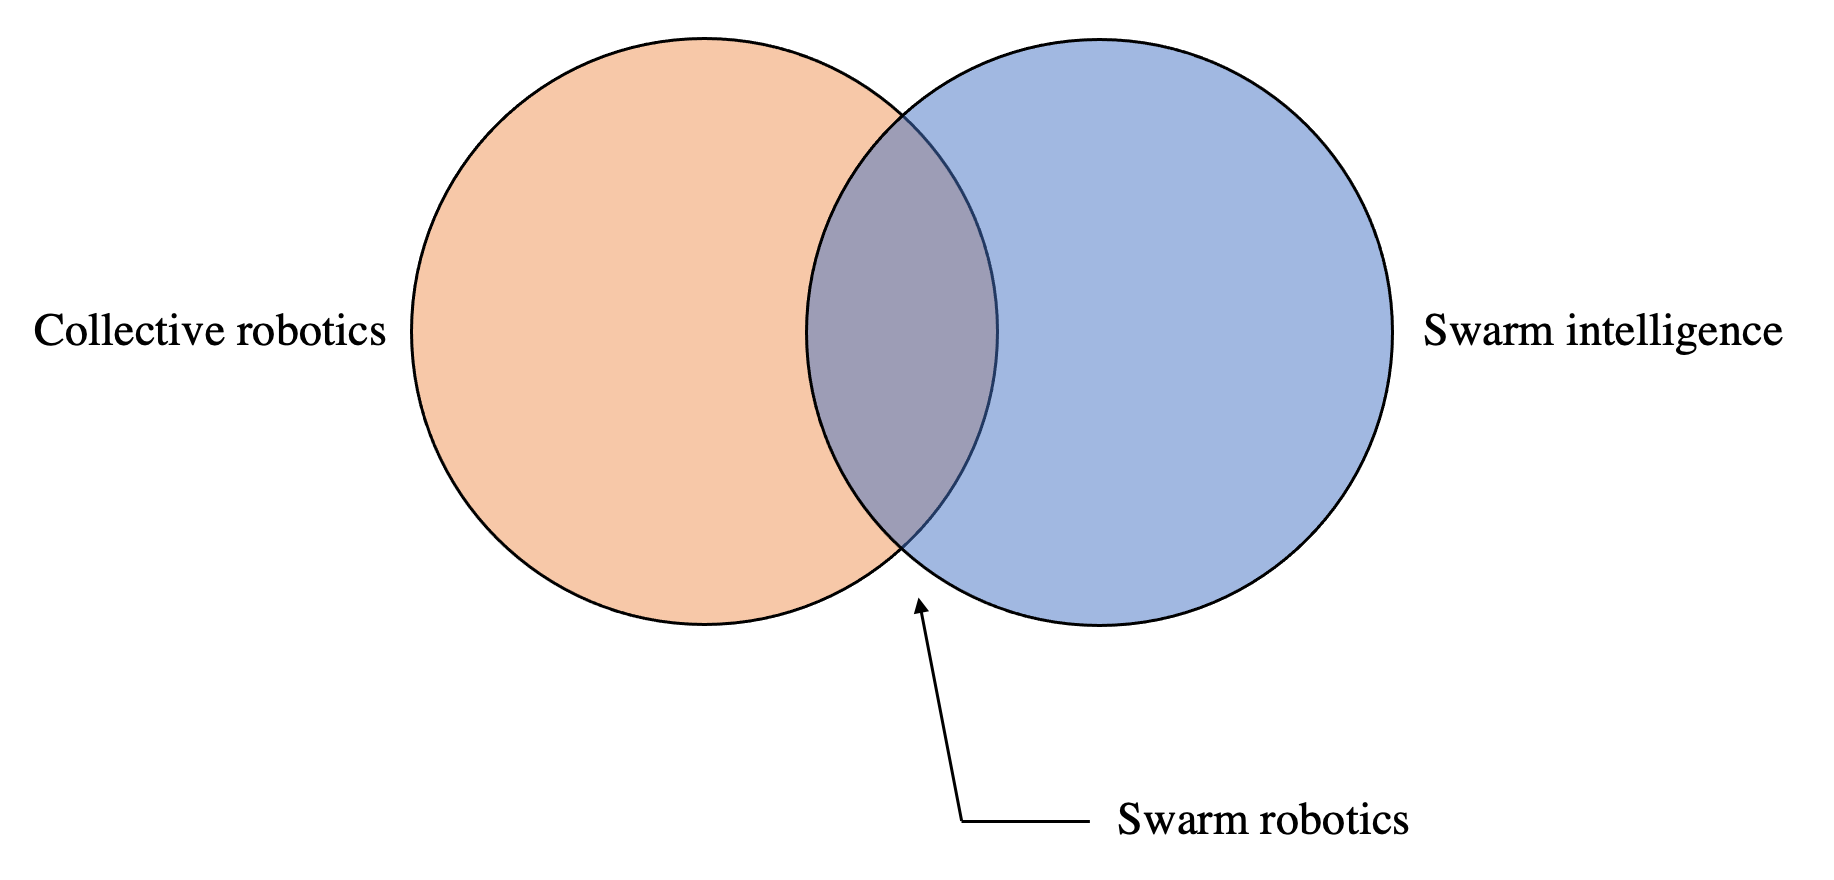
\includegraphics[width=0.99\columnwidth]{images/vennes.png}
    \caption{From natural to artificial swarm intelligence}
    \label{venne}
\end{figure}

The design principles of swarm robotic systems are the following: 

\begin{itemize}
    \item Decentralized control
    \item Absence of leadership
    \item Absence of predefined roles
    \item Simple and local interactions
\end{itemize}

Self-organization is achieved through local interactions between the robots of the system. Robots need to be aware of their neighbors and have the ability to communicate directly with them, or indirectly through environmental stimuli for example. Of course, because of the engineering nature of swarm robotics, physical limitations emerge. Bandwidth restrictions, communication capabilities, storage limitations and physical constraints all need to be taken into account when designing robot swarm systems.

\subsection{Stigmergy}
In nature, stirgmergy is a mechanism of indirect communication between agents of a system. It uses the environment for storing information that can be sensed and used by others. Stigmergy can be observed in social insects, for example ants that communicate between each other by laying pheromones on the ground to guide peers towards food \cite{bonabeau1999swarm}. Stigmergy is a fundamental aspect of swarm intelligence as it enables self-organization through local interactions.

The virtual stigmergy presented in \cite{pinciroliTuple2016} and implemented in the Buzz programming language \cite{pinciroliBuzz2016} achieves consensus among
a group of robots using Conflict-free Replicated Data Types (CRDTs), represented as key-value pairs shared and replicated among the swarm members.  It is a valuable tool for easily programming swarm behaviors and is specifically designed to meet the requirements of such robotic systems. 

\subsection{Belief Maps}
Belief maps are commonly used in exploration algorithms. They render a continuous surface into a discrete set of cells which is especially useful for engineering problems. Indeed, it allows highlighting specific regions of the environment and allows the designer of the algorithm to tune the level of precision at which the environment is represented. A finer granularity will provide a more accurate representation of the environment and as a result should offer more precision. However, finer granularity usually comes with higher computational costs. 

The cells of the belief map are used to store information about the corresponding surface they represent. For example, it could store the absence or presence of a specific feature. In this case, because it is portraying a binary feature, the belief map is referred as an occupancy map. In belief maps, the value associated with the cell is a probability and indicates the confidence level to which the cell is believed to contain a specific feature.

\subsection{Risk}
Recently, a lot of attention from the research community has been oriented towards risk-aware autonomous systems. Taking risk and uncertainty into account when designing robot systems is of capital importance as they are increasingly deployed on real-world scenarios with safety-critical applications, including the transportation sector, aerospace systems or collaborative manufacturing. They evolve in uncontrolled environments and must face risks on a regular basis, motivating the need for risk awareness. Excessive risk taking, or a complete absence of considering it, may not only jeopardize the robotic system, it may also endanger components in its vicinity and possibly human lives. For robot swarms tasked with the exploration of unknown environments, risk is generally location-based and takes the form of environmental hazards. 


\section{Problem Elements}
The exploration of hazardous environments using teams of robots comes with its own set of advantages and constraints. Carrying the exploration mission with numerous robots should result in faster terrain coverage than in a single robot mission.  However, failures can considerably reduce the performance of the team and should therefore by avoided as much as possible. Not taking risk into account when exploring will inevitably lead to a decrease in performance of the team. This intuition, applied to a scenario of terrain coverage is presented in Figure \ref{statementDORA1} and \ref{statementDORA2}. In figure \ref{statementDORA1}, robots of the team start exploring the environment and gathering information about it. After a while, in figure \ref{statementDORA2}, robots start experiencing failures due to environmental hazards. The environmental hazards take the form of point radiation sources. Because of failures, the number of team members carrying the exploration mission decreases drastically. As a result, the exploration rate decreases and large portions of the environment remain uncovered. 

The intuition presented in figures \ref{statementDORA1} and \ref{statementDORA2} presents the problem statement of the exploration algorithm DORA-Explorer. DORA-Explorer tries to solve it by introducing a consciousness of risk in the motion control loop of the robots. Because carrying the exploration effort with numerous robots should result in faster terrain coverage, the algorithm should also respect the design principles of swarm robotics.

\begin{figure}[H]
	\centering
    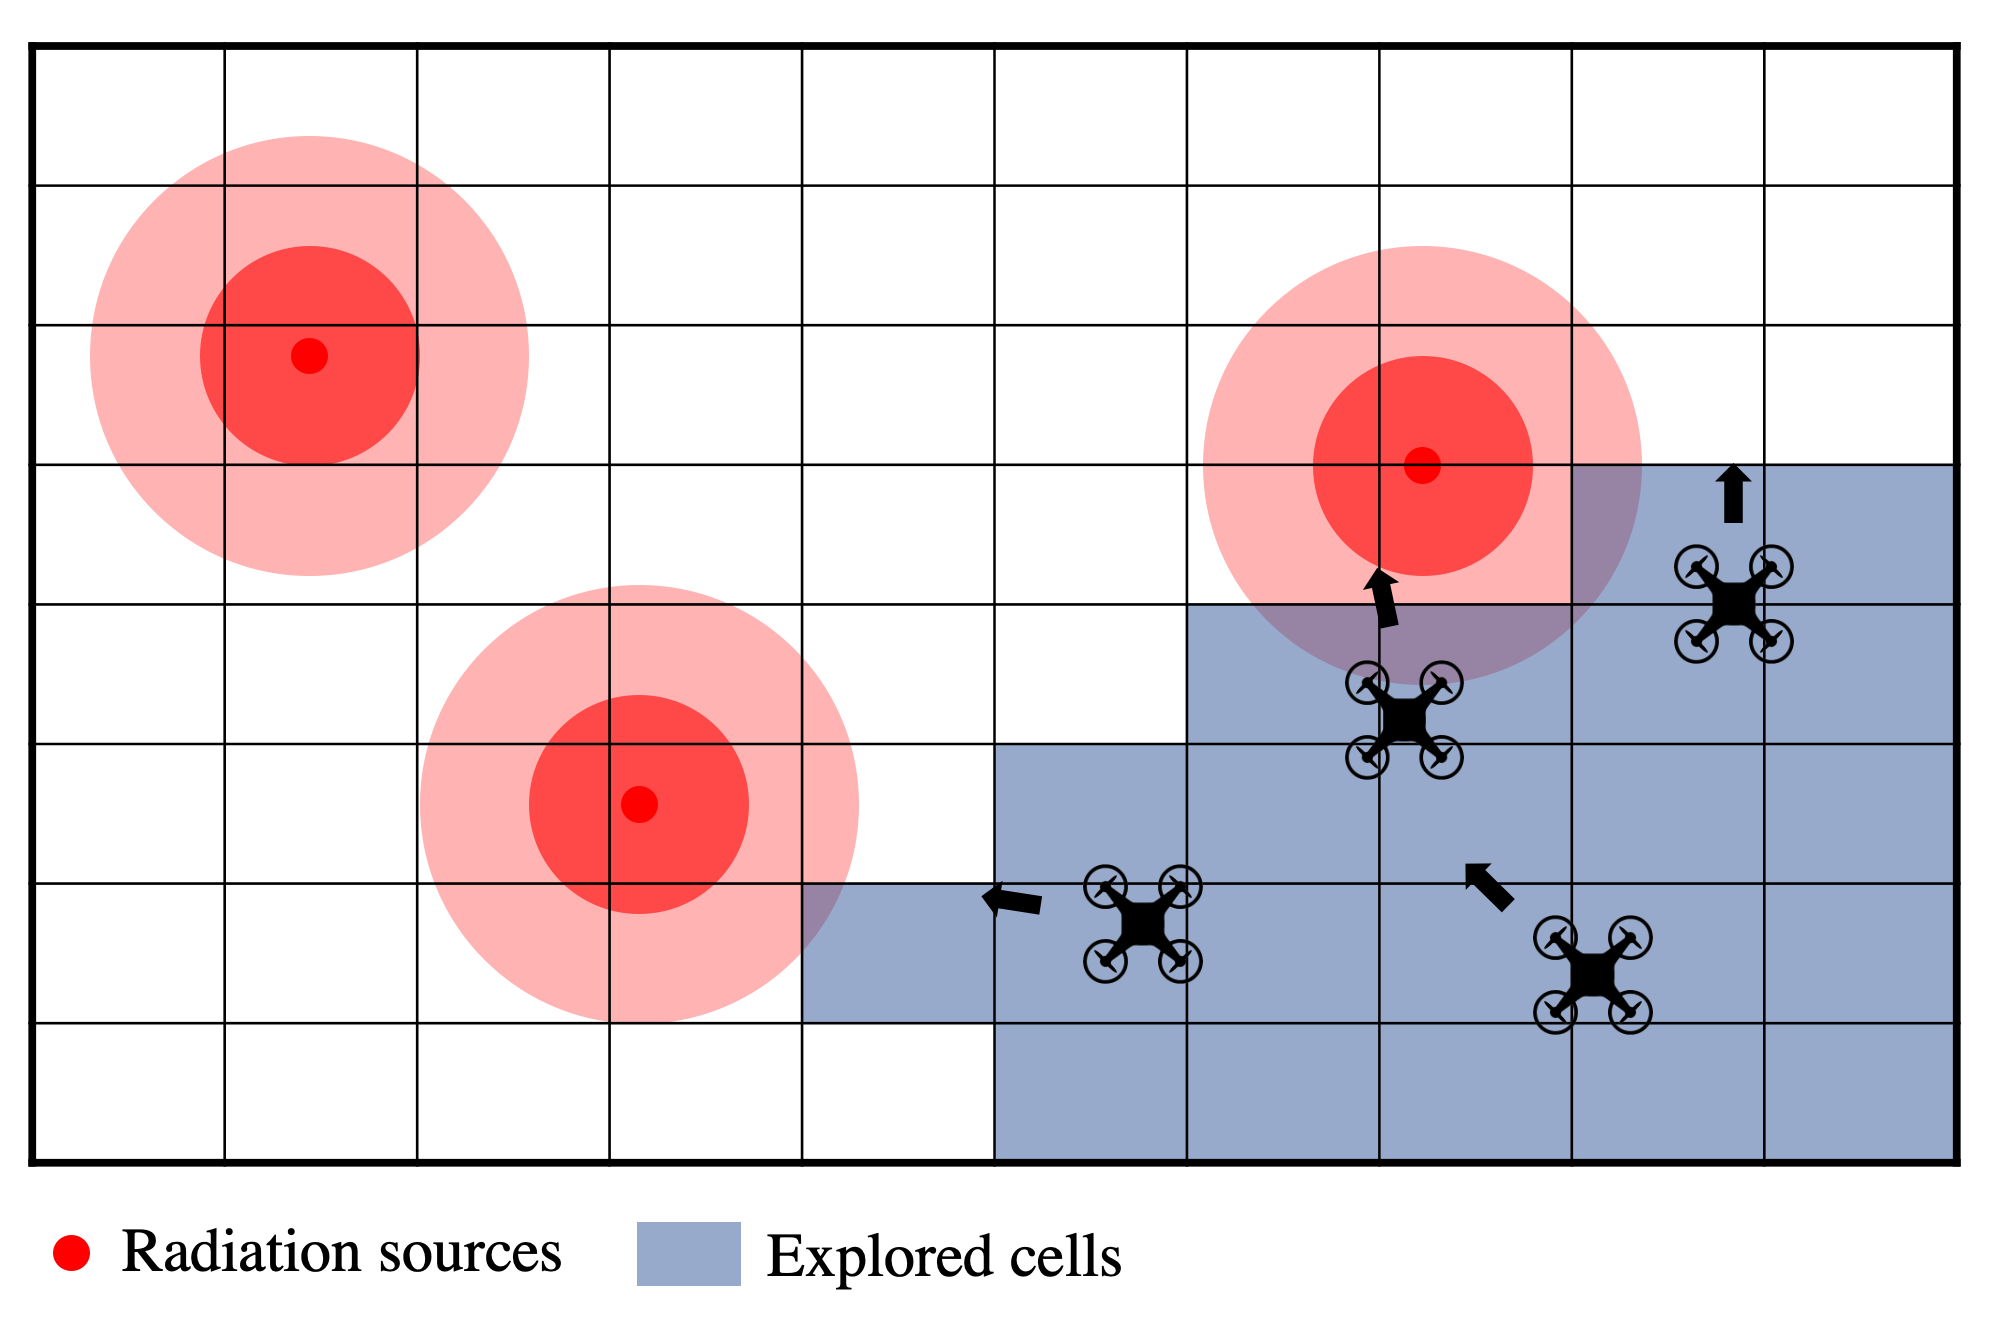
\includegraphics[width=0.85\columnwidth]{images/problemStatement1.png}
    \caption{Exploration of an unknown environment with a team of robots}
    \label{statementDORA1}
\end{figure}

\begin{figure}[H]
	\centering
    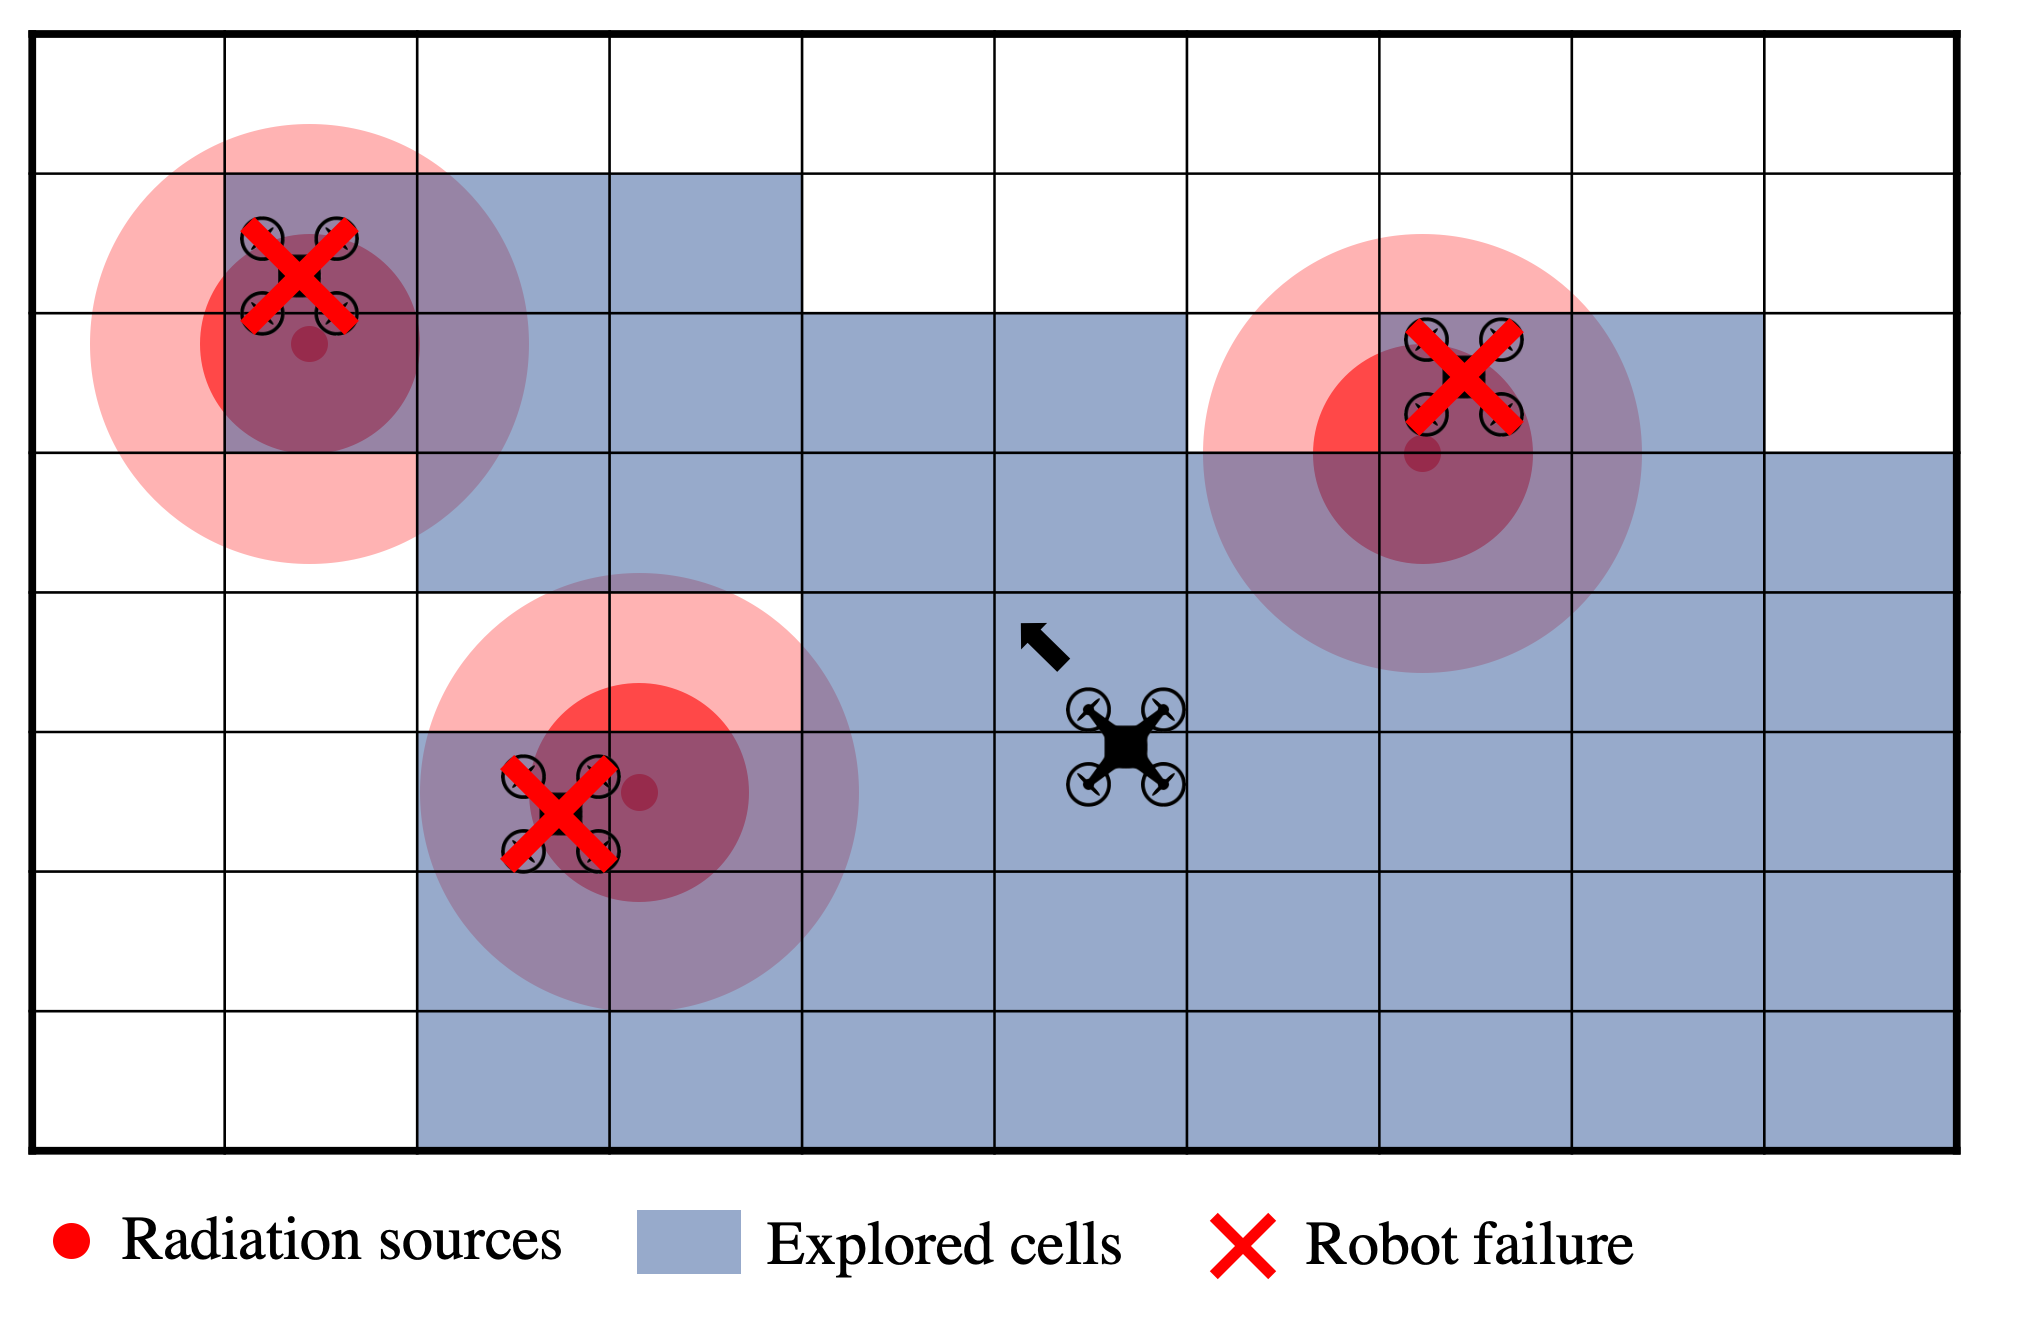
\includegraphics[width=0.85\columnwidth]{images/problemStatement2.png}
    \caption{Exploration of an unknown environment with a team of robots affected by failures.}
    \label{statementDORA2}
\end{figure}

% \begin{figure*}[h]
%     \centering
%     \begin{subfigure}{0.65\textwidth}
%         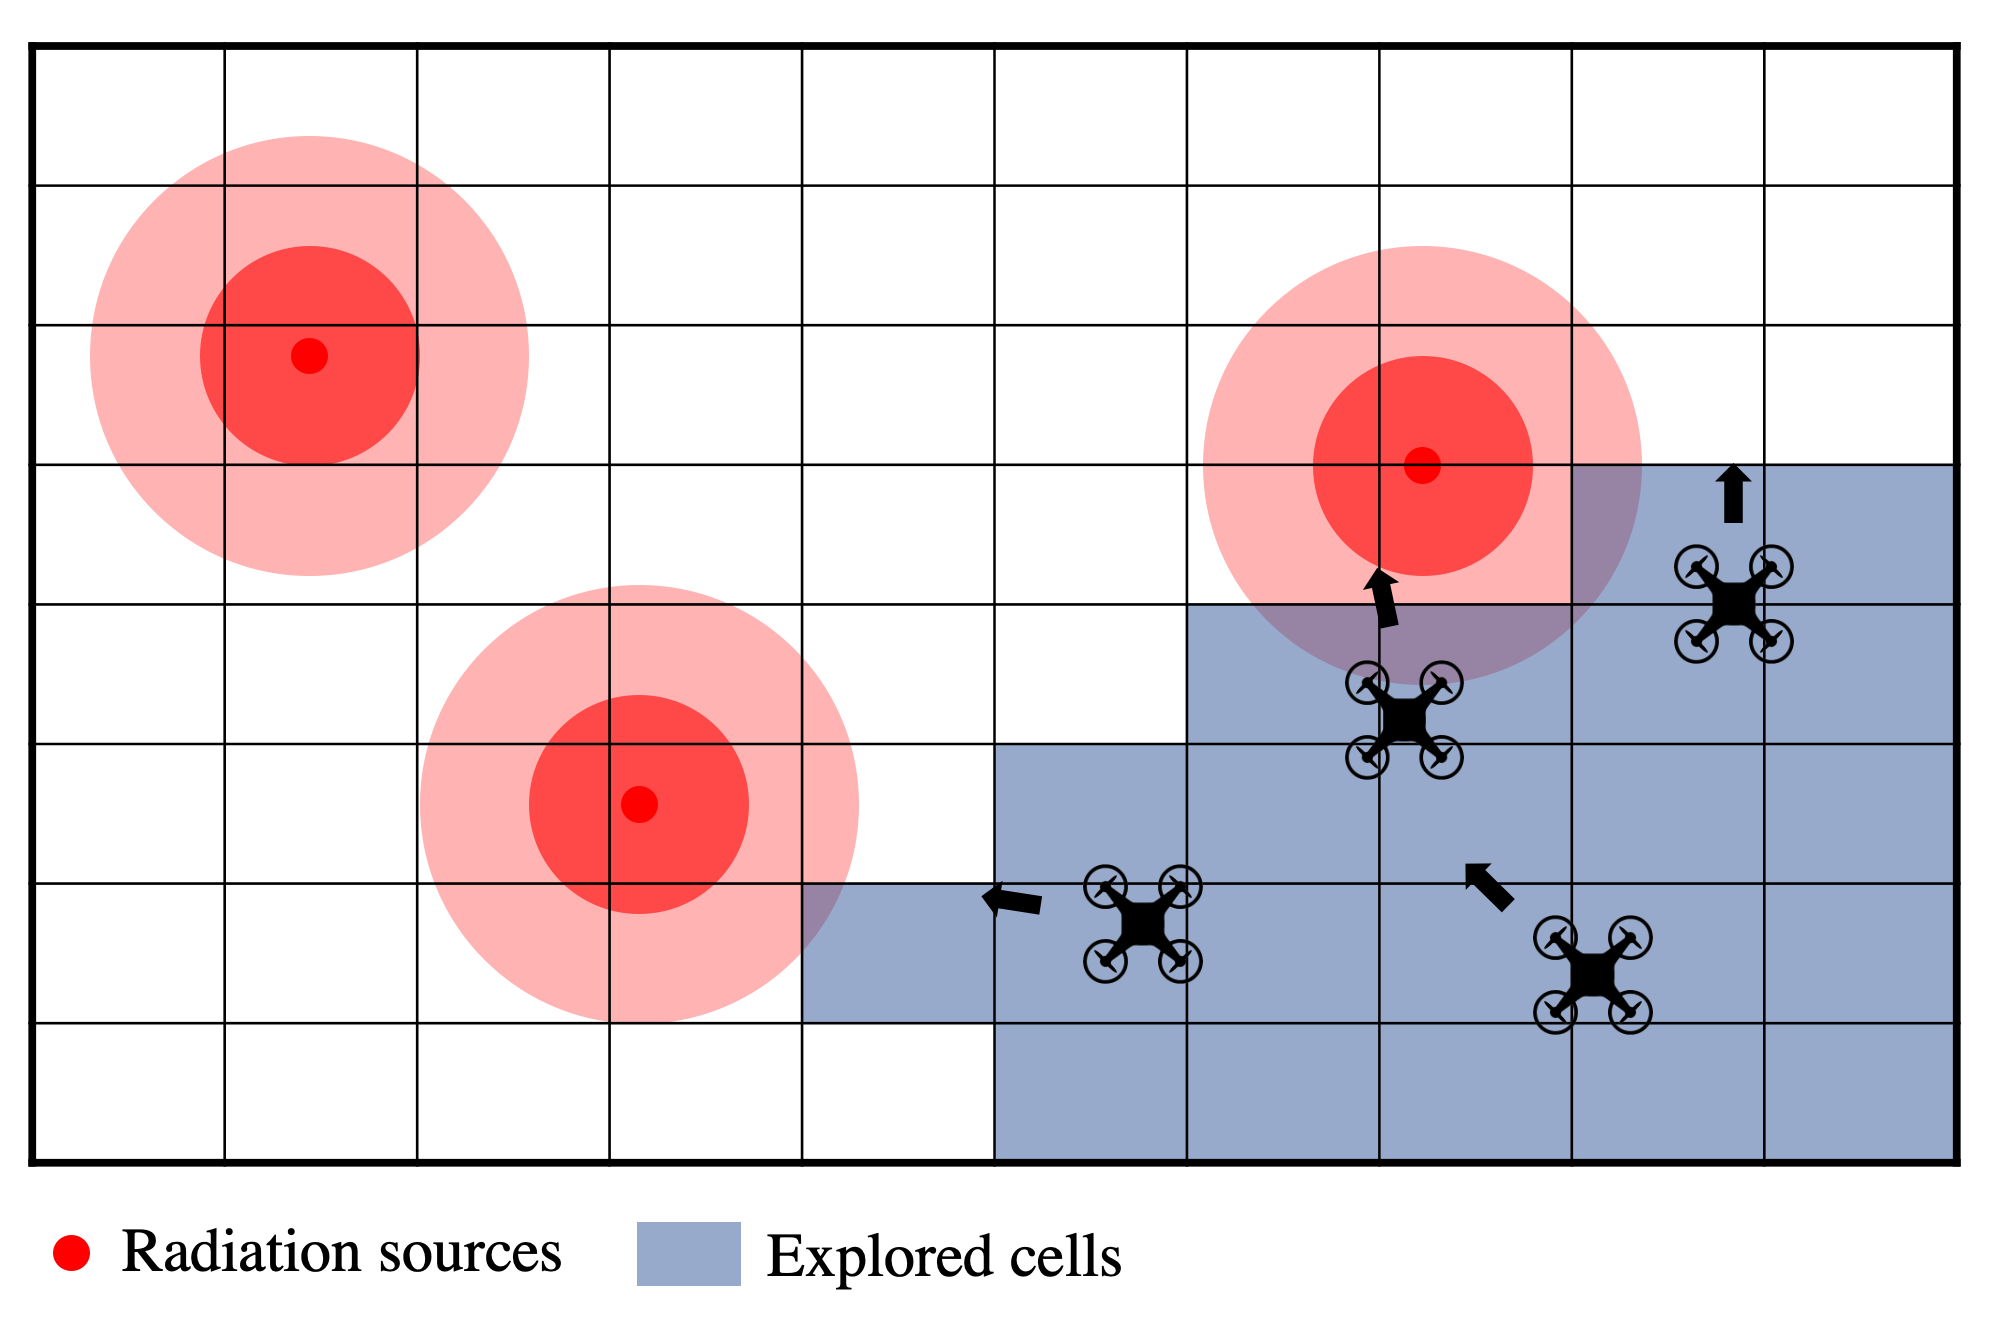
\includegraphics[width=\textwidth]{images/problemStatement1.png}
%         \caption{}
%         \label{statement1}
%     \end{subfigure}
%     \begin{subfigure}{0.65\textwidth}
%         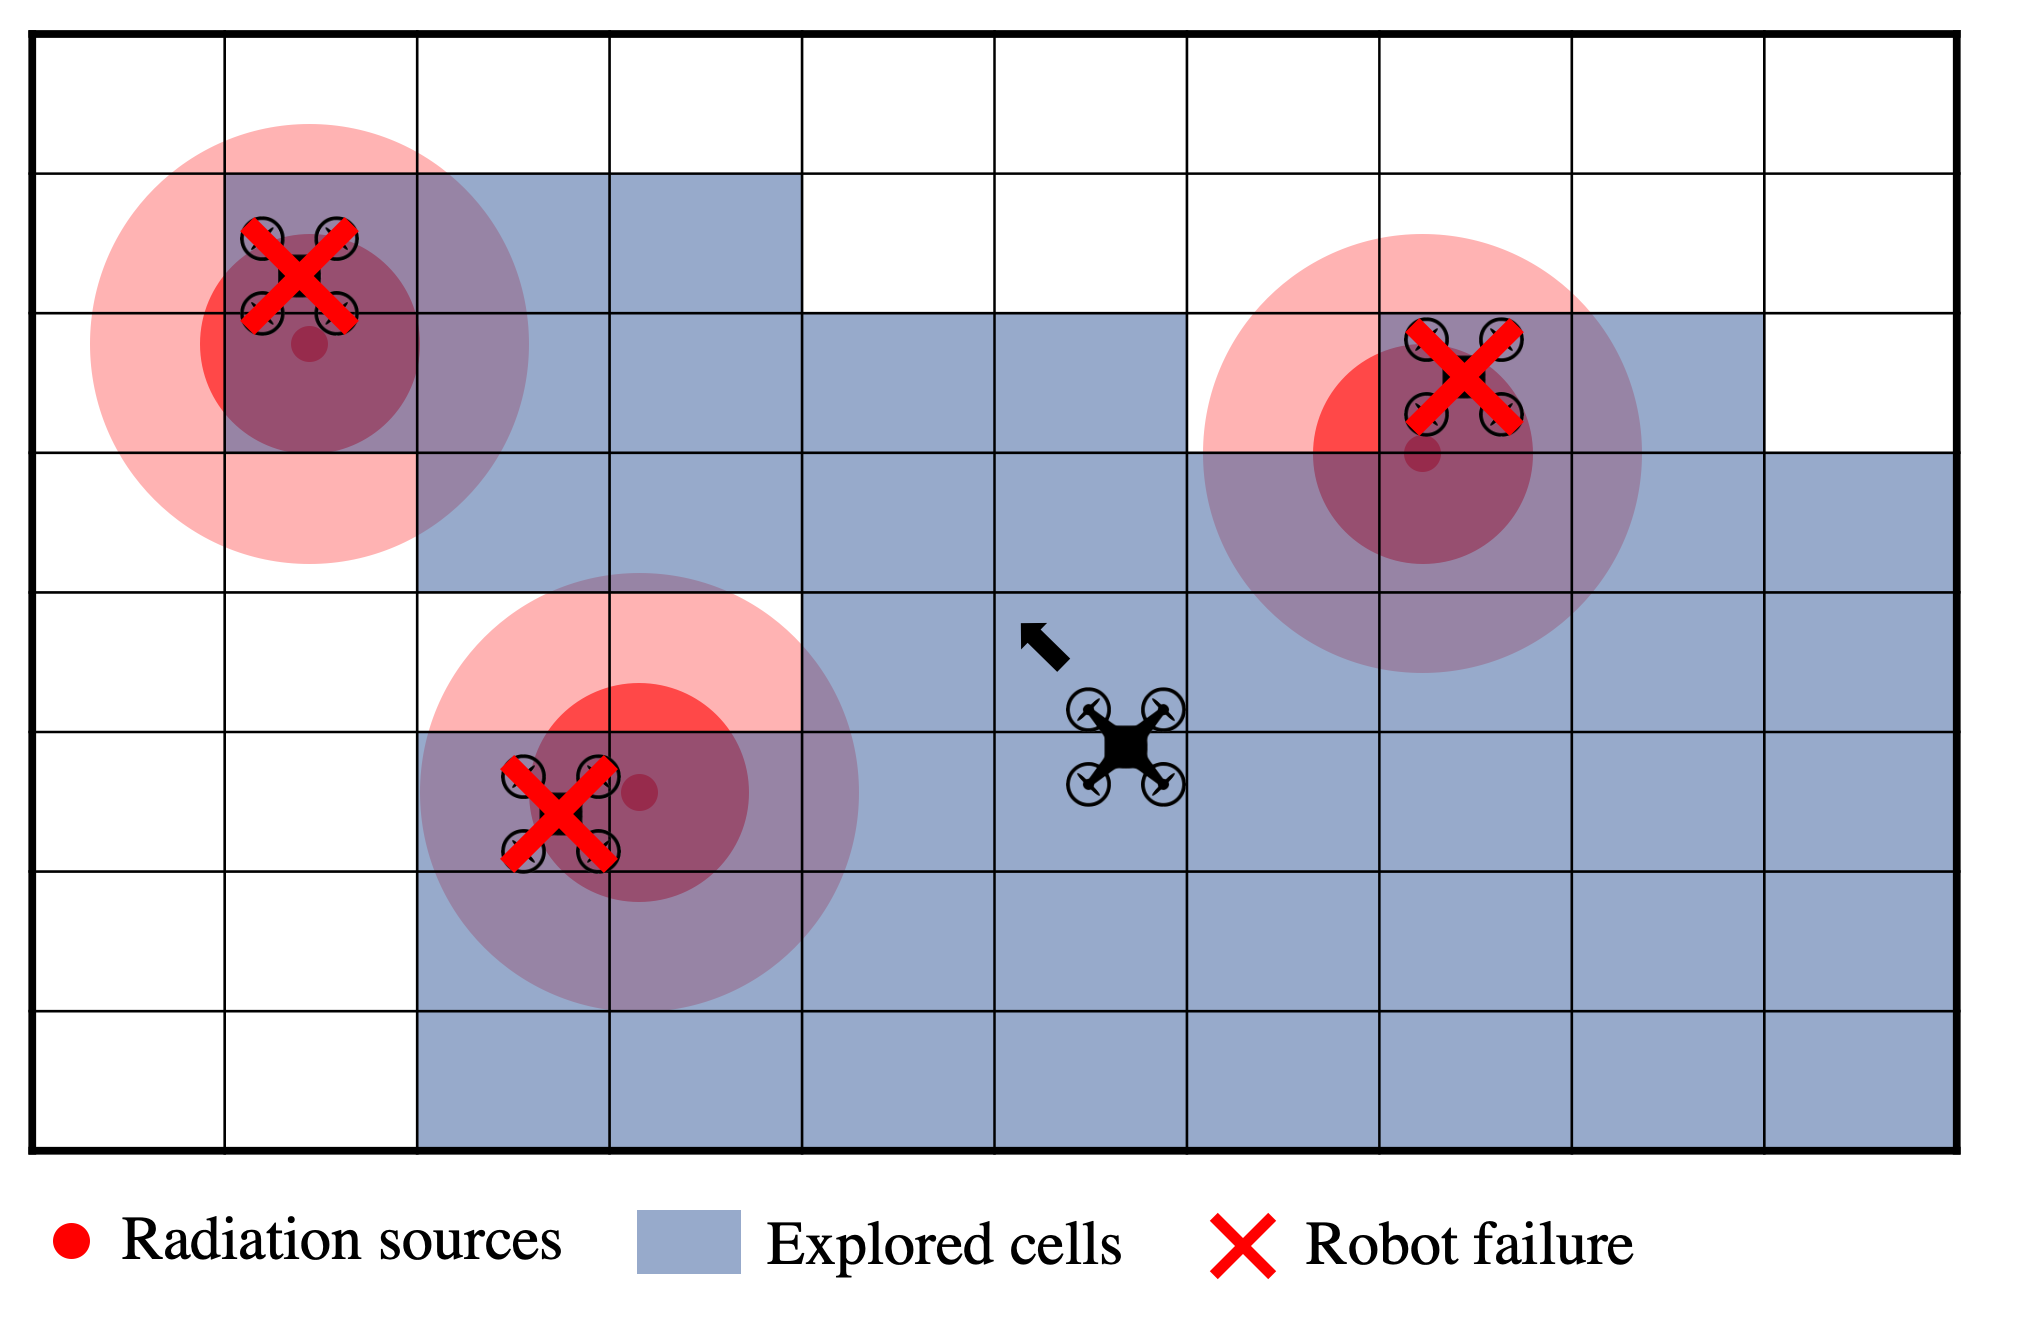
\includegraphics[width=\textwidth]{images/problemStatement2.png}
%         \caption{}
%         \label{statement2}
%     \end{subfigure}
%     \caption{Risk-unaware exploration: Exploring hazardous environments without considering risk.}
%     \label{statement}
% \end{figure*}


Naturally, a similar problem statement can be expressed in terms of information gathering. If robots collecting information about the explored terrain are susceptible to data corruptions, not taking risk into account will lead to poor data collection performance. This intuition is presented in Figure \ref{statementRASS}.

\begin{figure}[h]
	\centering
    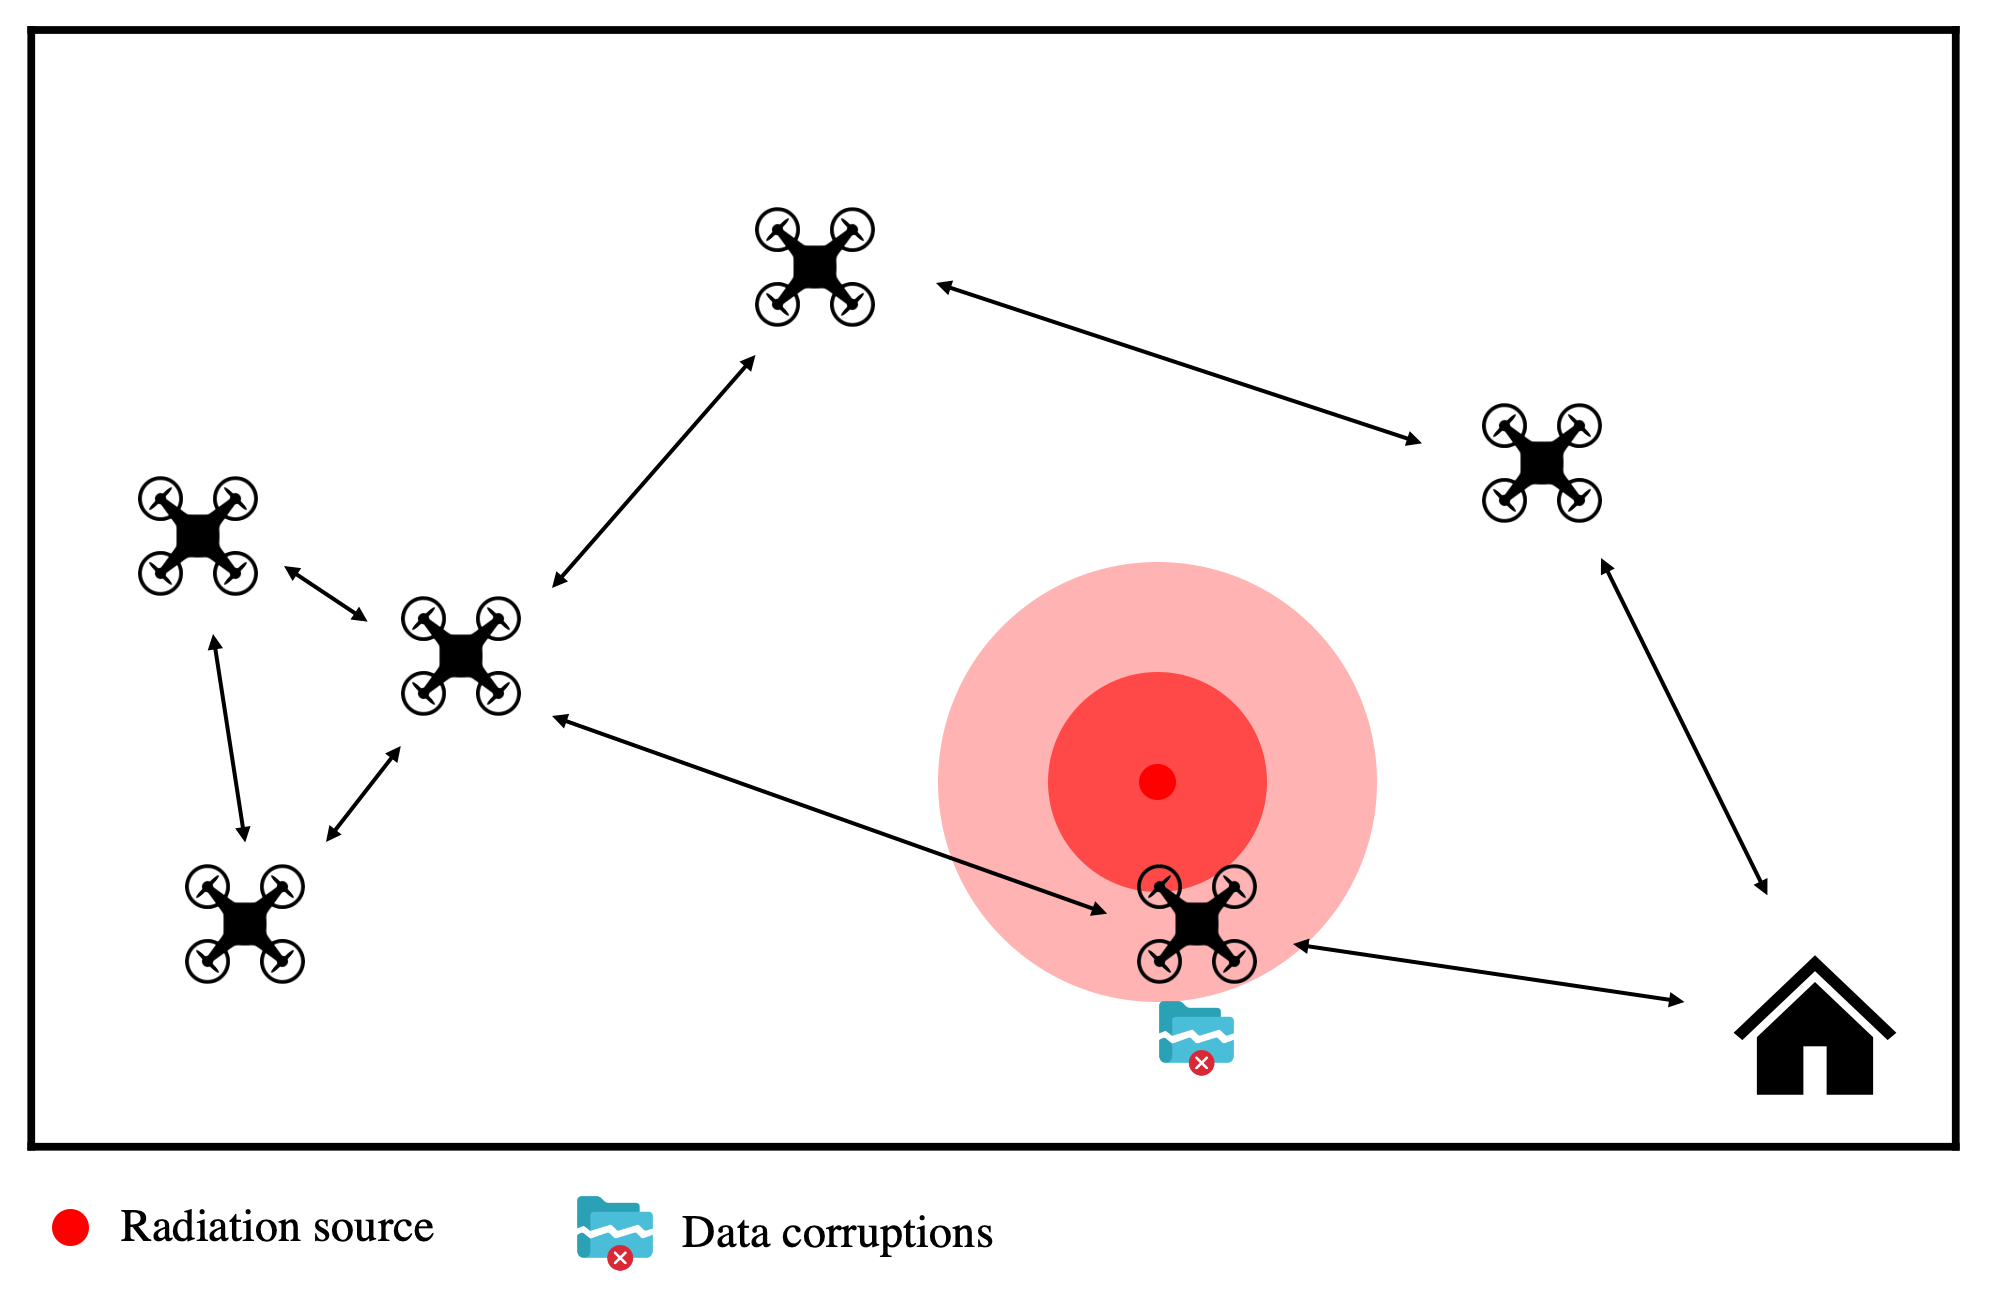
\includegraphics[width=0.95\columnwidth]{images/statementRASS.png}
    \caption{Information gathering in an hazardous environment}
    \label{statementRASS}
\end{figure}

In figure \ref{statementRASS}, robots are dispatched in an unknown environment with the task of gathering information about it. Because the environment contains dangers, in our case point radiation sources, data items collected by robots may become corrupted if exposed to radiations. Therefore, transiting collected data items through robots located near a radiation source will increase the likelihood of such corruptions. In figure \ref{statementRASS}, the lower route, although more direct towards the base station, is definitely more dangerous than the upper one. To avoid loosing data items, the robots should route the information towards the base station using the upper route. This is the problem statement of RASS, the second algorithm of the thesis. Using risk awareness, RASS solves the problem by avoiding risky nodes of the system in its storage and routing scheme.



\section{Research Objectives} 
\label{sec:objectifs}
The main research objective is bringing risk awareness to swarm algorithms used to perform exploration missions in hazardous environments. First, we focus on a risk-aware exploration algorithm, something that was lacking in the literature. Second, we focus on risk awareness at the storing and routing level of the swarm infrastructure. The research objectives are the following, the ones related to risk-aware exploration are first listed followed by the ones related to risk-aware storage and routing.


\subsection{Risk-aware exploration}
\begin{enumerate}
    \item Reduce failure rate compared to other state-of-the-art algorithms;
    \item Achieve comparable terrain coverage compared to other state-of-the-art algorithms;
    \item Respect swarm robotics design principles from section \ref{sec:designprinciples};
    \item Test real-world applicability with experiments on physical robots;
\end{enumerate}

\subsection{Risk-aware storage and routing}
\begin{enumerate}
    \item Reduce data corruption rate compared to other state-of-the-art algorithms;
    \item Achieve comparable transfer speed compared to other state-of-the-art algorithms;
    \item Respect swarm robotics design principles from section \ref{sec:designprinciples};
    \item Test real-world applicability with experiments on physical robots;
\end{enumerate}


\section{Thesis outline}
The remainder of the thesis is structured as follows. In chapter \ref{sec:RevLitt}, a literature review of relevant related works is presented. The following topics will be studied in the literature review: swarm robotics, swarm programming, information sharing, routing mechanisms, swarm exploration strategies, risk in swarm robotics and some notable fault detection methods. Following the literature review, in chapter \ref{sec:approach}, the scientific approach used to meet the research objectives will be presented. Then, in chapter \ref{sec:Theme1} the algorithm DORA-Explorer, which uses risk awareness in its exploration strategy, will be presented. Subsequently, chapter \ref{sec:Theme2} will cover RASS, a risk-aware storing and routing mechanism designed for robot swarms carrying exploration missions. A high-level discussion on the results obtained throughout the master's degree in relation with the research objectives will follow in chapter \ref{sec:discussion}. Finally, in chapter \ref{sec:Conclusion}, a conclusion is presented alongside the limitations of the work and interesting future research directions.
